\documentclass[a4paper]{article}

%use the english line for english reports
%usepackage[english]{babel}
\usepackage[portuguese]{babel}
\usepackage[utf8]{inputenc}
\usepackage{indentfirst}
\usepackage{graphicx}
\graphicspath{ {Images/} }

\usepackage{verbatim}
\usepackage{adjustbox}
\usepackage{hhline}
\usepackage{amsmath}
\usepackage{bm}
\usepackage{float}
\usepackage[T1]{fontenc}
\usepackage[colorlinks=true, allcolors=blue]{hyperref}
\usepackage{tikz}
\def\checkmark{\tikz\fill[scale=0.4](0,.35) -- (.25,0) -- (1,.7) -- (.25,.15) -- cycle;} 
\usepackage[a4paper,top=3cm,bottom=2cm,left=3cm,right=3cm,marginparwidth=1.75cm]{geometry}

\begin{document}

%\title{\Huge\textbf{Estudo de um Amplificador Operacional Discreto}\linebreak\linebreak\linebreak
%\linebreak
%
\includegraphics[scale=0.5]{feup_logo.png}
%\bigskip
%\bigskip
%\linebreak
%\Large{Mestrado Integrado em Engenharia Informática e Computação} \linebreak\bigskip\linebreak
%\huge{Electrónica 2}\linebreak
%}
%\vspace{2cm}
%\author{Mafalda Pereira Varela - up201403432 \\ António Tomás Costa Nunes - up201405099 \\ %\linebreak\medskip\linebreak \\
%\\ Faculdade de Engenharia da Universidade do Porto \\ Rua Roberto Frias, s/n, 4200-465 Porto, Portugal %\linebreak\linebreak\linebreak
%\linebreak\linebreak\vspace{3cm}}
%\date{Junho de 2007}
%\maketitle
%\thispagestyle{empty}

%\newpage

%************************************************************************************************
%************************************************************************************************
\title{
\includegraphics[scale=0.5]{feup_logo.png}\\
    \bigskip
    \bigskip
    \bigskip
    \bigskip
    \bigskip
    \bigskip
    \bigskip
    \bigskip
    \huge{Electrónica 2}\\
    \bigskip
    \bigskip
    \Huge\textbf{Estudo de um Amplificador Operacional Discreto}
}

\author{\\\bigskip\bigskip\bigskip\bigskip\bigskip\bigskip\bigskip\bigskip\bigskip\bigskip\bigskip\\
        Mafalda Pereira Varela - up201403432\\
        António Tomás Costa Nunes - up201405099}

\date{\bigskip\bigskip\textbf{Dezembro de 2016}}

\maketitle

\newpage

%\section*{Resumo}
%Resumo sucinto do trabalho com 150 a 250 palavras (problema abordado, objetivo, como foi o problema resolvido/abordado, principais %resultados e conclusões).

%************************************************************************************************
%************************************************************************************************

%************************************************************************************************
%************************************************************************************************
\tableofcontents

\newpage

%%%%%%%%%%%%%%%%%%%%%%%%%%
%\section{Introdução}

%Descrever os objetivos e motivação do trabalho. Descrever num parágrafo breve a estrutura do relatório.

%$V_B__Q_5$
%\clearpage

%%%%%%%%%%%%%%%%%%%%%%%%%%
\section{Dimensionamento e Simulação}
    \medskip
    \subsection{Dimensionamento do Amplificador}
        \bigskip
    Para o dimensionamento do amplificador teve-se em conta que as correntes em todos os transistores se têm de situar entre $1mA$ e $3mA$ e que a excursão de saída varia entre $-8V$ e $+8V$, como indicado no guião.
        
        Tendo já algumas resistências predefinidas prosseguiu-se ao cálculo das indefinidas, considerando também que terão de ser aproximadas à série E12.
        
        \begin{itemize}
            \item \textbf{R2 --} Começamos por ter em conta a excursão máxima que nos coloca $8,7V$ na base do transistor $Q_5$ e coletor de $Q_3$, a queda emissor-coletor em $Q_3$ tem de ser no mínimo $0,3V$, deixando uma margem de mais $0,7V$ consideramos uma tensão de $9,7V$ no emissor de $Q_3$. Atendendo agora à corrente máxima e mínima em cada transistor optamos por uma corrente de aproximadamente $2m5A$ em $Q_3$, menor que o máximo $3mA$, o que nos coloca em $Q_1$ e em $Q_2$ correntes de $1,25mA$. Tendo isto podemos calcular a resistência $R_2$ da seguinte forma:
            $$R_2 = \frac{12-9,7}{1,25\times10^{-3}} = 1k84\ \Omega \Rightarrow \bm{1k8\ \Omega} \Rightarrow I_{Q1} = I_{Q2} = 1,28mA$$
            
            \item \textbf{R3 --} Tendo uma corrente em $Q_2$ de $1,28mA$, e considerando a corrente de $Q_3$ de aproximadamente $1,5mA$ calculamos $R_3$ da seguinte forma:
            $$R_3 = \frac{12-9,7}{1,28\times10^{-3} + 1,5\times10^{-3}} = 827\ \Omega \Rightarrow \bm{820\ \Omega} \Rightarrow I_{Q3} = 1,52mA$$
            
            \item \textbf{R5 \& R6 --} Como consideramos $9,7V$ no emissor de $Q_3$ e a queda emissor-base $0,7V$, obtemos $9V$ como tensão de base de $Q_3$. Considerando a relação de tensões em $R_5$ ($12V\rightarrow9V$) e $R_6$ ($9V\rightarrow0V$) concluímos que $R_6$ tem de ter o triplo do valor de $R_5$, devendo estas ser bastante mais baixas que $r_{\pi_{Q3}}$ de forma a aumentar o ganho do transistor.
            $$\beta_{Q3} = \beta_P = 330$$
            
            $$Gm_{Q3} = \frac{I_{Q3}}{V_t} = \frac{1,5\times10^{-3}}{25\times10^{-3}} = 60m\frac{A}{V}$$
            
            $$r_{\pi_{Q3}} = \frac{\beta_{Q3}}{Gm_{Q3}} = 5k5 \Omega$$
            
            Com $r_{\pi_{Q3}}=5k5\Omega$ podemos então arbitrar os valores $R_6 = \bm{1k\Omega}$ e $R_5 = \bm{330\Omega}$. Temos também de ter em conta que a potência de cada resistência não pode ultrapassar os $250mW$.
            $$P_{R6} = \frac{V^2}{R_6} = 81mW < 250mW\ \checkmark$$
            Portanto estas resistências estão corretamente dimensionadas!
            
            \item \textbf{R7 \& R8 --} De forma a dimensionar as resistências $R_7$ e $R_8$ fizemos os seguintes cálculos, a tensão no coletor de $Q_3$, que é igual à de base de $Q_5$ em máxima excursão tem o valor de $+8,7V$, enquanto que a do coletor de $Q_7$, ou seja a de base de $Q_6$ em excursão máxima encontra-se nos $-8,7V$, assim:
            $$R_7 + R_8 = \frac{8,7 - (-8,7)}{1\times10^{-3}} = 17k4\Omega$$
            
            $$R_7 = R_8 = 8k7\Omega \Rightarrow \bm{8k2\Omega}$$
            
            \item \textbf{R12 --} Tendo a tensão na base de $Q_7$ como $-9V$ e a queda de tensão base-emissor de $0,7V$ obtemos a tensão no emissor de $-9,7V$, sabendo também que a corrente em $Q_7$ é a mesma que em $Q_3$, pois as correntes de base de $Q_5$ e $Q_6$ são aproximadamente nulas, facilmente calculamos $R_{12}$:
            $$R_{12} = \frac{-9,7 - (-12)}{1,5\times10^{-3}} = 1k53\Omega \Rightarrow \bm{1k5\Omega}$$
            
            \item \textbf{R13 \& R14 --} Devido à simetria do circuito concluímos que as resistências $R_{13}$ e $R_{14}$ podem ser dimensionadas da mesma forma que $R_5$ e $R_6$, logo $R_{13} = R_6 = \bm{1k\Omega}$ e $R_{14} = R_5 = \bm{330\Omega}$.\\
            
            \item \textbf{R16 --} Finalmente, dimensionamos $R_{16}$ da seguinte forma, sabendo que a corrente em $Q_8$ é a soma das correntes de $Q_1$ e $Q_2$, temos a corrente de $Q_8$ aproximadamente igual a $2,56mA$, sabemos também a tensão no emissor de $Q_8$, a mesma que no emissor de $Q_7$, como sendo $-9,7V$ o que nos permite calcular a soma de $R_{15}$ e $R_{16}$:
            $$R_{15} + R_{16} = \frac{-9,7 - (-12)}{2,56\times10^{-3}} = 898\Omega \Rightarrow R_{16} = \bm{680\Omega}$$
            De forma a obter a soma das resistências desejada podemos ajustar o potênciometro $R_{15}$ para aproximadamente $\bm{220\Omega}$\\
            \smallskip
        \end{itemize}
        
        \begin{table}[H]
            \centering
            \hspace*{-0,7cm}\begin{tabular}{|c|c|c|c|c|c|c|c|c|c|c|c|c|c|c|c|}\hline
            $R_1$ & $\bm{R_2}$ & $\bm{R_3}$ & $R_4$ & $\bm{R_5}$ & $\bm{R_6}$ & $\bm{R_7}$ & $\bm{R_8}$ & $R_9$ & $R_{10}$ & $R_{11}$ & $\bm{R_{12}}$ & $\bm{R_{13}}$& $\bm{R_{14}}$ & $R_{15}$ & $\bm{R_{16}}$\\\hhline{|-|-|-|-|-|-|-|-|-|-|-|-|-|-|-|-|}
            $100k$ & $\bm{1k8}$ & $\bm{820}$ & $100k$ & $\bm{330}$ & $\bm{1k}$ & $\bm{8k2}$ & $\bm{8k2}$ & $100$ & $22$ & $22$ & $\bm{1k5}$ & $\bm{1k}$& $\bm{330}$ & $\approx220$ & $\bm{680}$\\\hline
            \end{tabular}
            \caption{\label{tab:resistencias}Lista das Resistências do OpAmp em Ohm}
        \end{table}
        \medskip
    
    %%%%%%%%%%%%%%%%%%%%%%%%%%
    \subsection{Excursão, polarização e ganho em malha aberta}
        \bigskip
        Tendo já o AmpOp dimensionado, é agora necessário dimensionar as resistências $R_{f1}$ e $R_{f2}$ de forma a que o ganho em malha fechada seja de $-100 \frac{V}{V}$, podemos então fazê-lo da seguinte forma:
        $$\frac{V_o}{R_{f2}} = -\frac{V_i}{R_{f1}} \Leftrightarrow \frac{V_o}{V_i} = -\frac{R_{f2}}{R_{f1}} = -100 \Leftrightarrow R_{f2} = 100\times R_{f1}$$
        
        $$R_{f1} = \bm{1k\Omega}\qquad \qquad \quad R_{f2} = \bm{100k\Omega}$$ 
        
        Através da simulação do circuito conforme indicado na figura 3 do guião, a leitura do ganho em malha aberta é de $\bm{23572,6 \frac{V}{V}}$.
        \begin{figure}[H]
            \centering
            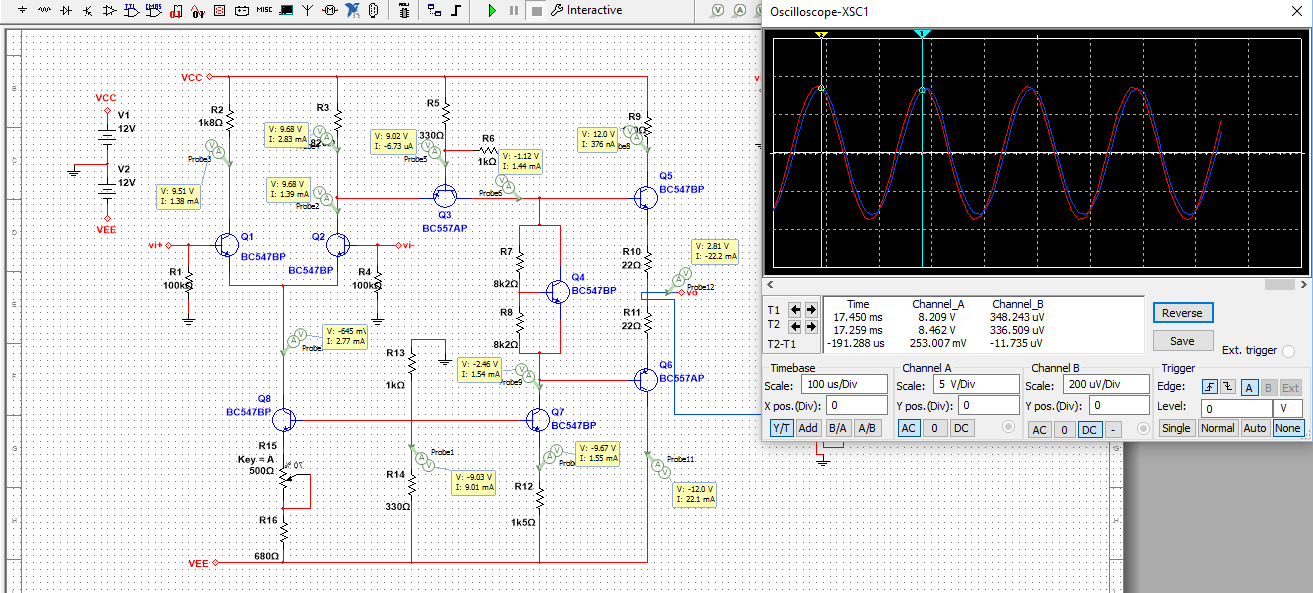
\includegraphics[width=\textwidth]{figura1_multisim.png}
            \caption{\label{fig:ganhoMultisim}Leitura do ganho em malha aberta através de simulação}
        \end{figure}
        \bigskip
    
    %%%%%%%%%%%%%%%%%%%%%%%%%%
    \subsection{Montagem e soldadura dos componentes na placa de circuito impresso}
        \medskip
        \begin{figure}[H]
        \centering
        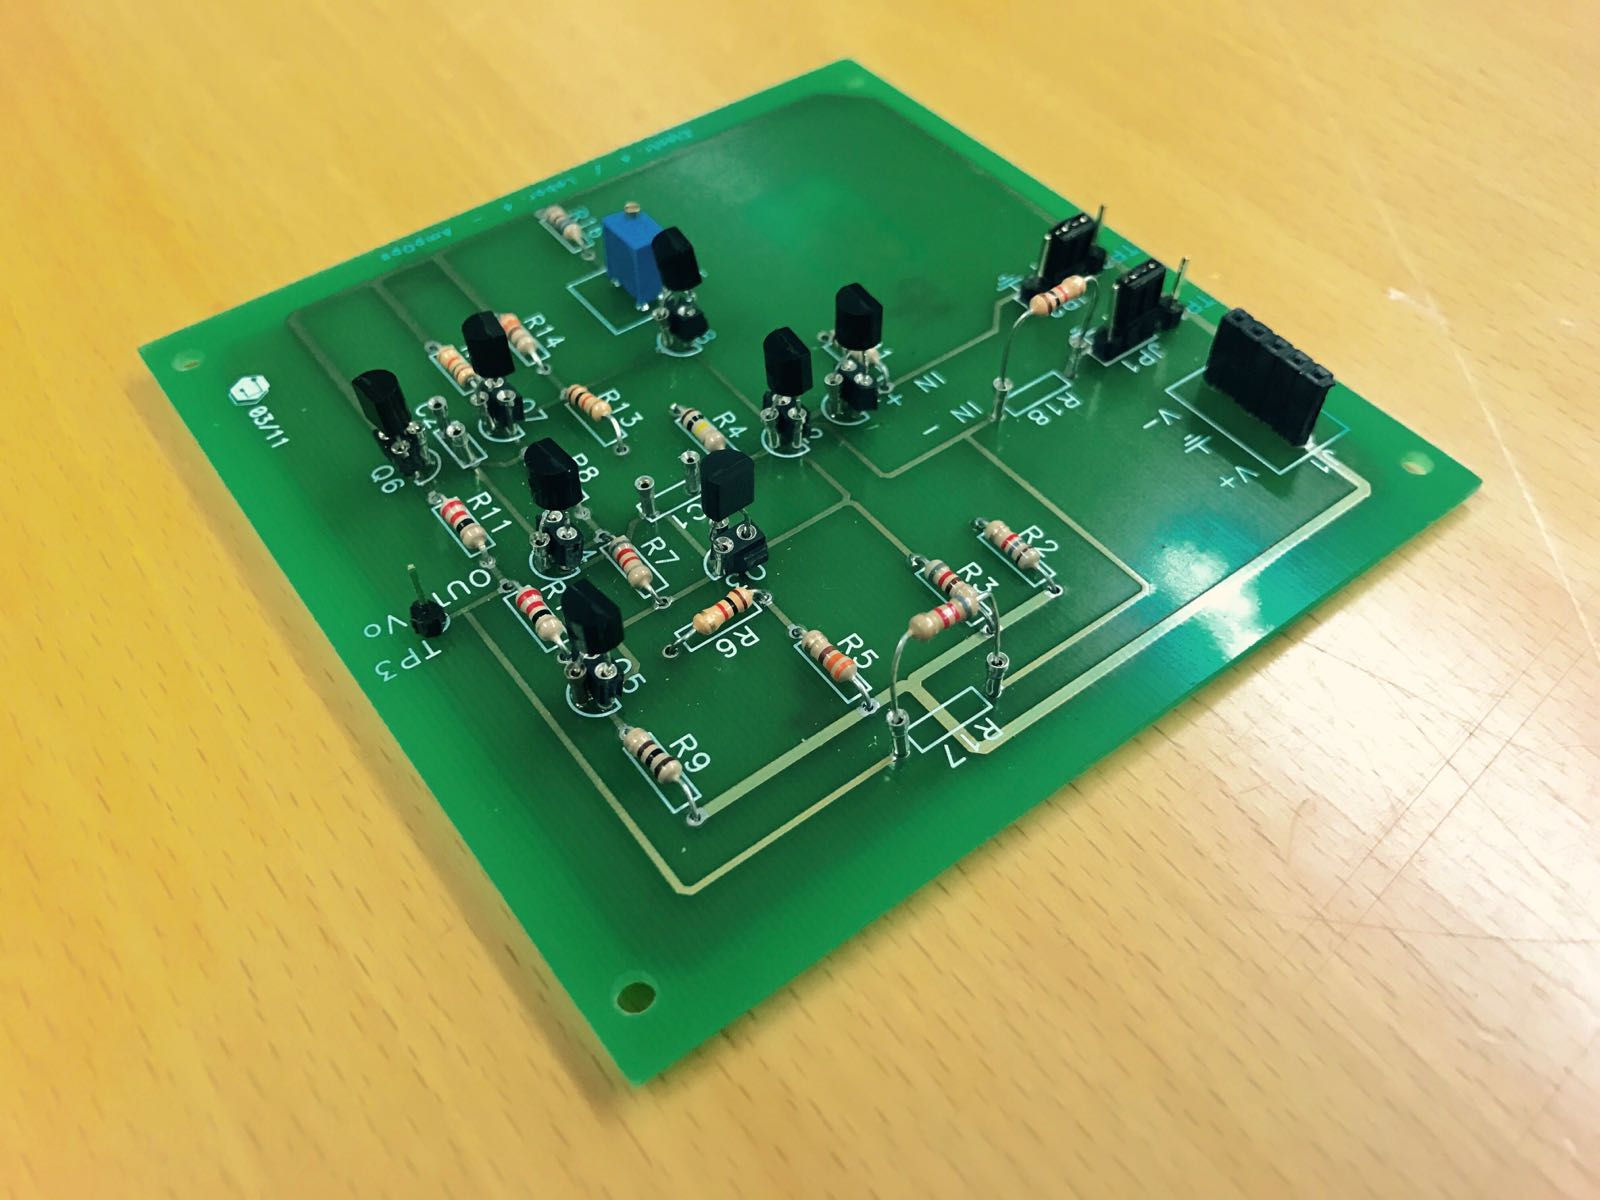
\includegraphics[width=\textwidth]{figura2_circuito_soldado.jpeg}
        \caption{\label{fig:circuitoSoldado}Leitura do ganho em malha aberta através de simulação}
        \end{figure}
        
\clearpage

%%%%%%%%%%%%%%%%%%%%%%%%%%
\section{Medição das principais grandezas associadas à polarização, tensão de desvio à entrada e ganho em malha aberta do operacional}
    \bigskip
    \subsection{Medidas de polarização}
        \medskip
        Depois de regular $R_{15}$ de acordo com o calculado anteriormente e de fazer pequenos ajustes de forma a obter a corrente desejada em $R_{16}$, as tensões e correntes em regime permanente são as seguintes:
        \begin{figure}[H]
            \centering
            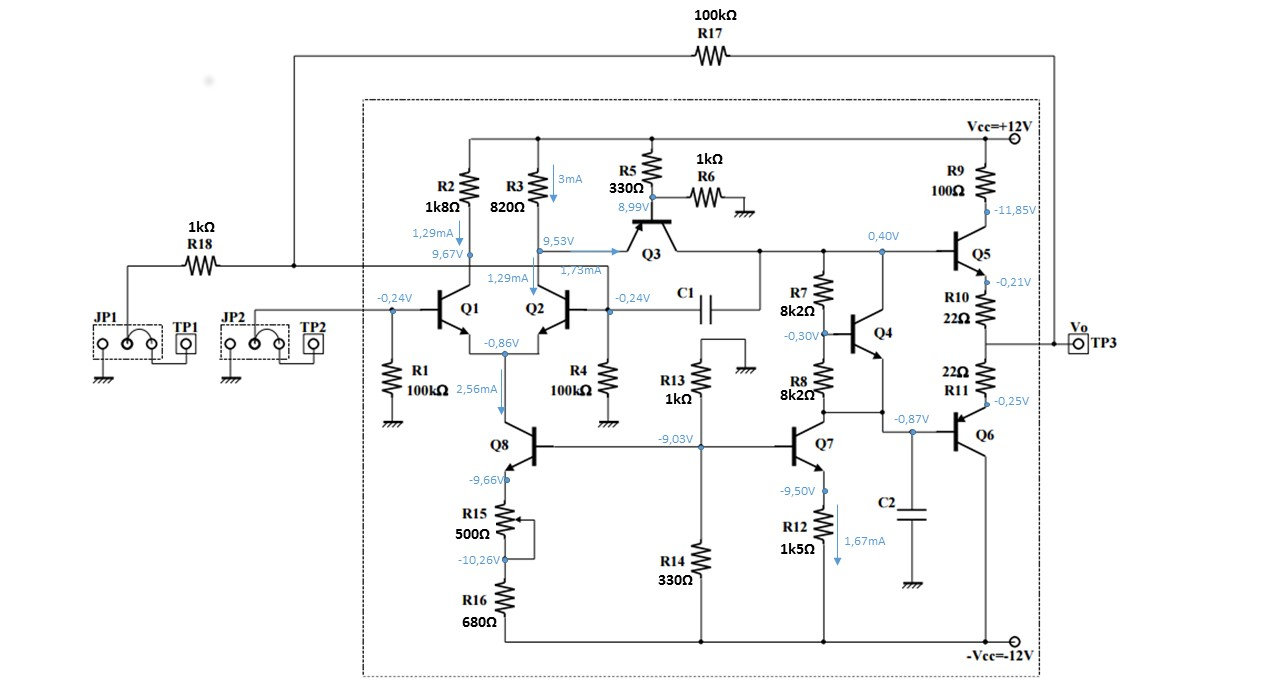
\includegraphics[width=\textwidth]{figura3_tensoesCorrentesDC.jpg}
            \caption{\label{fig:tensoesCorrentesDC}Tensões e correntes em regime permanente}
        \end{figure}
        \smallskip
    
    %%%%%%%%%%%%%%%%%%%%%%%%%%
    \subsection{Medidas de desvio à entrada e ganho}
        \bigskip
        De forma a analisar a tensão de desvio à entrada $V_{ios}$ (offset) e o ganho em malha aberta, $A$, é retirado $R_{17}$ e curto-circuitado $R_{18}$ é ainda colocado o amplificador operacional num circuito conforme a figura abaixo (retirada do guião).
        \begin{figure}[H]
            \centering
            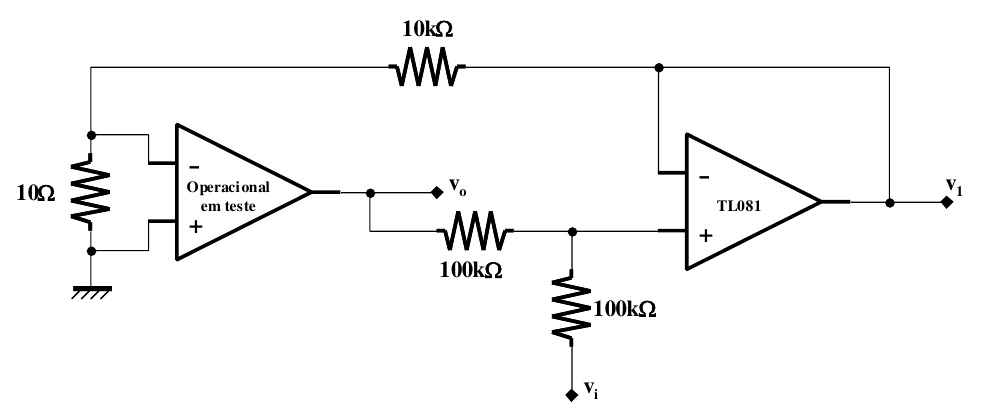
\includegraphics[width=\textwidth]{figura4_circuitoTeste.png}
            \caption{\label{fig:cicuitoTeste}Circuito de teste da tensão de desvio e ganho em malha aberta (figura retirada do guião)}
        \end{figure}
        \medskip
        
        \subsubsection{Estudo da montagem da Figura 4}
            \bigskip
            Começando por "retirar"\ a fonte de tensão de \emph{offset} para fora do nosso amplificador operacional e considerando-o como ideal ficamos com uma tensão $V_{ios}$ no terminal $V_{i-}$ do mesmo, tendo isto, facilmente chegamos a:
            $$\frac{V_{ios}}{10} = \frac{V_1 - V_{ios}}{10k} \Leftrightarrow \frac{V_1}{1k} = (V_{ios} + \frac{1}{1k}V_{ios})1k \Leftrightarrow \bm{V_1 = 1001\times V_{ios}}$$
            
            Considerando agora os dois \emph{OpAmps} como ideais, a tensão ao terminal $V_{i-}$ do nosso como sendo $\frac{V_o}{A}$ e aplicando um sinal em $V_i$, podemos concluir que a tensão no terminal $V_{i-}$ do amplificador \verb|TL081| tem o valor de $V_1$. A partir disto conseguimos obter:
            $$\frac{\frac{V_o}{A}}{10} = \frac{V_1 - \frac{V_o}{A}}{10k} \Leftrightarrow \frac{V_o}{A}\times (1k + 1) = V_1 \Leftrightarrow V_o = \frac{V_1\times A}{1001}$$
            
            $$\frac{V_o - V_1}{100k} = \frac{V_1 - V_i}{100k} \Leftrightarrow V_1\times(\frac{A}{1001} - 1) = V_1 - V_i \Leftrightarrow \frac{A}{1001} = 1 + \frac{V_1}{V_1} - \frac{V_i}{V_1} \Leftrightarrow A = 1001\times (2 - \frac{V_i}{V_1})$$
            
            Sendo que em malha aberta ligamos o sinal de entrada ao terminal $V_{i+}$ o ganho será o inverso, logo $\bm{A = 1001\times (\frac{V_i}{V_1} - 2)}$            
            \medskip
        
        \subsubsection{Cálculo de desvio à entrada (\emph{Offset})}
            \medskip
            Colocando $V_i = 0V$ obtém-se $V_{ios} = V_1\times1001$, como visto na alíne anterior.
            
            Por medição obtemos que $V_i = -10,41V$, o que implica um $V_{ios} = \bm{-10,39mV}$.
            \medskip
        
        \subsubsection{Cálculo do ganho em malha aberta}
            \medskip
            Para o cálculo em malha aberta foi aplicado um sinal sinusoidal $V_i$ com uma tensão de aproximadamente $1V$ e com uma frequência de $5kHz$. Como verificado no ponto 2.2.1 o ganho é dado por $A=1001\times(\frac{V_i}{V_1} - 2)$.
        
            \begin{enumerate}
                \item De forma a substituir o transistor $Q_7$ por uma resistência que mantenha a corrente em $Q_3$ é necessário que:
                $$R_{12} + R_{Q7} = \frac{-0,87-(-12)}{1,5\times10^{-3}} = 7420\Omega$$ 
                $$R_{Q7} = 5920\Omega \Rightarrow \bm{5k6\Omega}$$
                
                Substituindo então $Q_7$ por uma resistência de $5k6\Omega$ entre os terminais coletor-emissor obtemos o seguinte ganho:
                \begin{figure}[H]
                    \centering
                    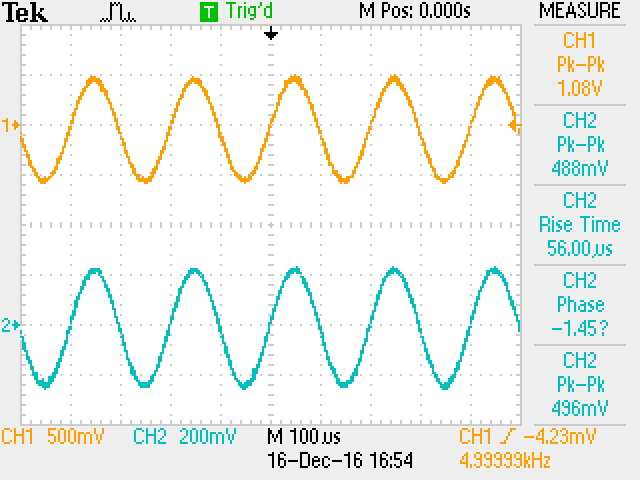
\includegraphics[width=0.5\textwidth]{figura5_ganhoResistencia.JPG}
                    \caption{\label{fig:ganhoComResistencia}Ganho com resistência de $5k6\Omega$ entre o coletor e emissor de $Q_7$}
                \end{figure}
                \centerline{$A = 1001\times(\frac{1,08}{0,488} - 2) = \bm{177,59\frac{V}{V}}$}
                \bigskip
                
                \item Mantendo a resistência da alínea anterior, mas acrescentando agora um condensador de $10\ \mu F$ entre o $V_o$ e o emissor de $Q_7$ obteve-se o seguinte:
                \begin{figure}[H]
                    \centering
                    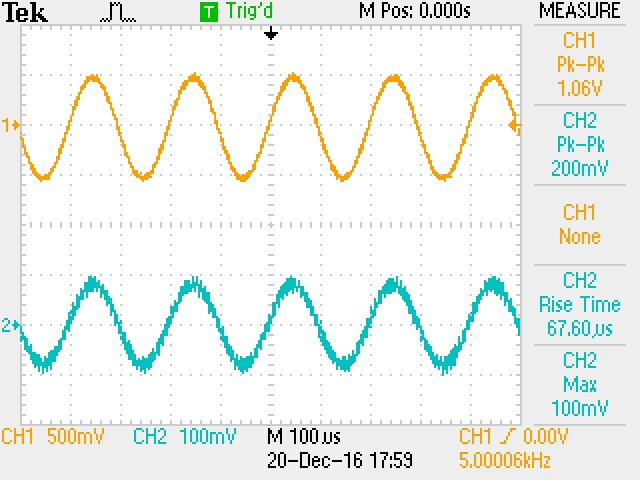
\includegraphics[width=0.5\textwidth]{figura6_ganhoCondensador.JPG}
                    \caption{\label{fig:ganhoComCondensador}Ganho com adição de um condensador de $10\ \mu F$ entre o $V_o$ e o emissor de $Q_7$}
                \end{figure}
                \centerline{$A = 1001\times(\frac{1,08}{0,2} - 2) = \bm{3303,3\frac{V}{V}}$}
                \bigskip
                
                Devido ao efeito de \emph{bootstrap} existe uma melhoria do ganho, uma vez que é aplicado parte do sinal de saída à entrada de modo a aumentar o valor da resistência.
                \bigskip
                            
                \item Repondo as características do circuito inicialmente em análise, retirando condensador e resistência e repondo $Q_7$ verificou-se:
                \begin{figure}[H]
                    \centering
                    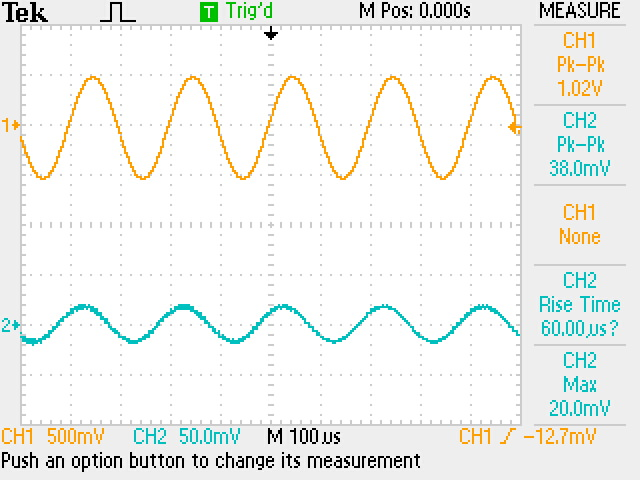
\includegraphics[width=0.5\textwidth]{figura7_ganhoMalhaAberta.JPG}
                    \caption{\label{fig:ganhoMalhaAberta}Ganho do OpAmp em malha aberta}
                \end{figure}
                \centerline{$A = 1001\times(\frac{1,08}{38\times10^{-3}} - 2) = \bm{24866,9\frac{V}{V}}$}
                \bigskip
                
	            Verificamos agora que o ganho aumenta significativamente quando é utilizado o transistor $Q_7$. Tal acontece pois ao utilizar uma resistência como carga, se pretendermos aumentar o ganho é necessário aumentar o seu valor, o que diminui a corrente, o que não nos interessa, e pode até levar os transistores a sair da sua zona de saturação, é possível melhorar substancialmente a situação substituindo a resistência por um transistor, neste caso $Q_7$, que atua como carga ativa para $Q_3$.
                \bigskip
            \end{enumerate}
        
\clearpage

%%%%%%%%%%%%%%%%%%%%%%%%%%
\section{Estudo da Resposta em Frequência do Amplificador}
    \medskip
    \subsection{Determinação da largura de banda}
        \bigskip
        Após a aplicação uma onda quadrada de frequência de $10kHz$ e de $228mV$ de amplitude,verificou-se que não havia saturação e a resposta temporal na saída do circuito encontra-se na figura abaixo:
        \begin{figure}[H]
            \centering
            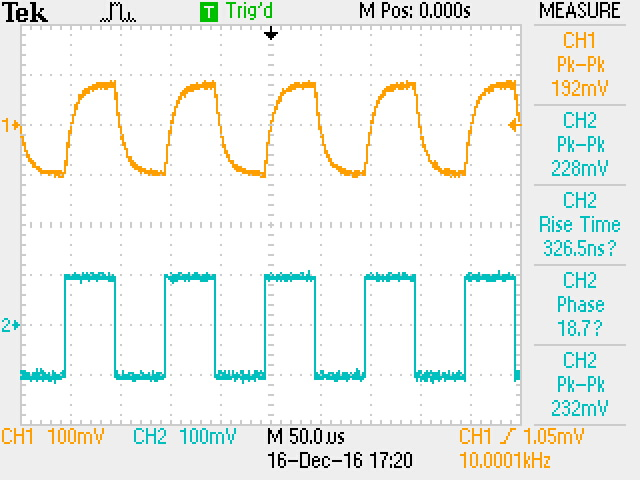
\includegraphics[width=0.5\textwidth]{figura8_respostaTemporal.JPG}
            \caption{\label{fig:respostaTemporal}Resposta temporal do circuito}
        \end{figure}
        \medskip
        
        A frequência superior de corte (pólo dominante) da montagem é dada por $f_H\times t_r = 0,35$, sendo $f_H$ a frequência superior de corte e $t_r$ o tempo de subida (entre os $10\%$ e $90\%$) que neste circuito corresponde a \bm{$168,4 ns$}, como podemos verificar pelo gráfico abaixo. Assim, o valor da frequência superior de corte é de \bm{$2,07MHz$}.
        \begin{figure}[H]
            \centering
            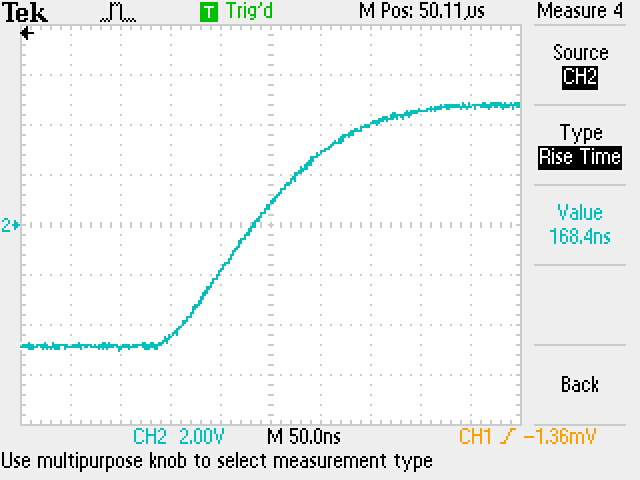
\includegraphics[width=0.5\textwidth]{figura9_tempoSubida.JPG}
            \caption{\label{fig:tempoSubida}Tempo de subida do circuito em malha fechada}
        \end{figure}
        \medskip
        
        É agora possível obter a frequência superior de corte (pólo dominante) em malha aberta, $f_{H_{ma}}$, usando os resultados recolhidos anteriormente através da seguinte expressão $f_{H_{ma}}\times A_{ma} = A_{mf}\times f_{H_{mf}}$. Onde $f_{H_{mf}}$ é a frequência superior de corte em malha fechada $(2,07MHz)$, $A_{ma}$ o ganho em malha aberta $(24866.9\frac{V}{V})$ e $A_{mf}$ o ganho em malha fechada $(-100\frac{V}{V})$.
        $$f_{H_{ma}} = \frac{100\times 2,07\times 10^6}{24866,9} = \bm{8,3kHz}$$
        
        Em malha aberta apresenta um valor muito reduzido de frequência de corte, como esperado devido à relação dos ganhos, interessando-nos então apenas em malha fechada de modo a termos uma larga banda de frequências.
    
    %%%%%%%%%%%%%%%%%%%%%%%%%%
    \subsection{Estudo da Estabilidade e Compensação}
        \bigskip
        Começamos por alterar a resistência $R_{17}$ para $10k\Omega$ de modo que o ganho em malha fechada seja de $-10\frac{V}{V}$, de seguida testamos diferentes valores de resistências para $R_{17}$ de modo a obter um forte ringing, mas sem oscilação. Como podemos ver na figura 10, a resistência que melhor se adequou ao desejado foi a $\bm{8k2\Omega}$, que provoca um ganho de $-8,2\frac{V}{V}$.
        \begin{figure}[H]
            \centering
            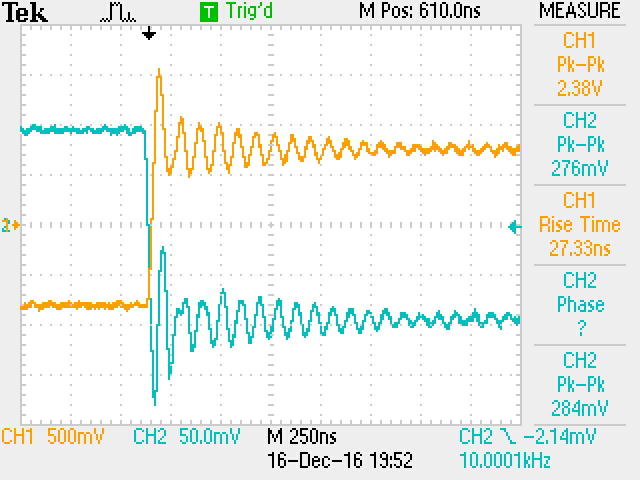
\includegraphics[width=0.5\textwidth]{figura10_respostaRinging.JPG}
            \caption{\label{fig:respostaRinging}Resposta com forte \emph{ringing}, sem oscilação, usando $Q_7$ como $8k2\Omega$}
        \end{figure}
        \medskip
        
        Após testar vários valores para $C_1$ na ordem dos $pF$ e $nF$ chegamos à conclusão que o condensador que origina a melhor resposta ao degrau, com um tempo de subida de $\bm{434.0ns}$, tem o valor de $\bm{27pF}$. 
        \begin{figure}[H]
            \centering
            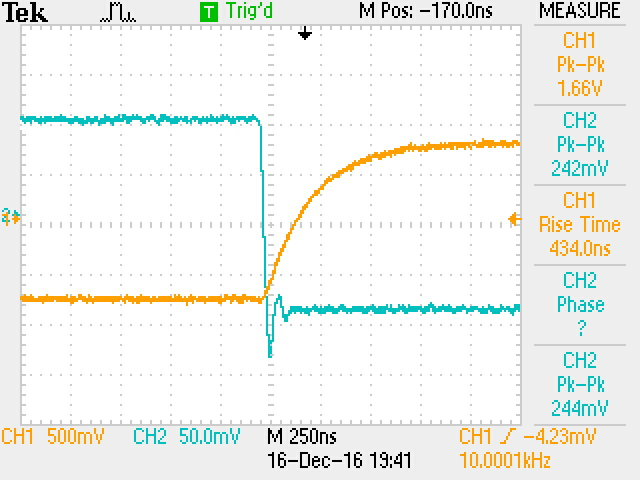
\includegraphics[width=0.5\textwidth]{figura11_respostaC1.JPG}
            \caption{\label{fig:respostaC1}Resposta sobre-amortecida devido à adição de $C_1$}
        \end{figure}
        \medskip
        
        Seguindo o mesmo processo para $C_2$ chegamos à conclusão que o melhor tempo de subida que conseguimos obter é de $\bm{224.0ns}$, com um condensador de $\bm{180pF}$. 
        \begin{figure}[H]
            \centering
            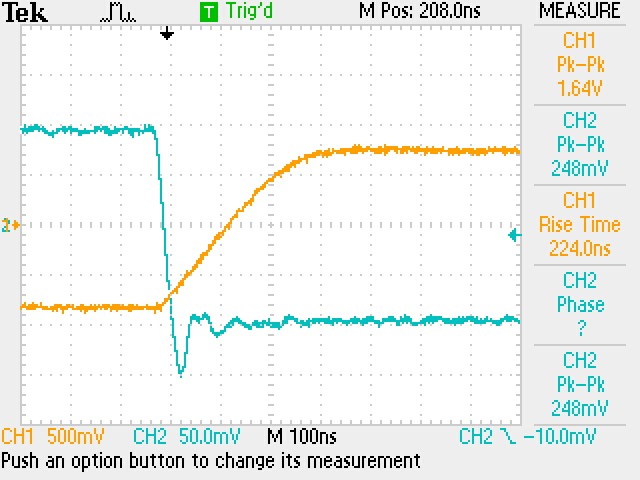
\includegraphics[width=0.5\textwidth]{figura12_respostaC2.JPG}
            \caption{\label{fig:respostaC2}Resposta sobre-amortecida devido à adição de $C_2$}
        \end{figure}
        \medskip
        
        Verificou-se assim que embora seja necessário que o condensador $C_2$ tenha um valor mais elevado que $C_1$ de forma a provocar os mesmos efeitos, inclusive a eliminação do efeito de \emph{ringing}, $C_2$ consegue produzir uma melhor resposta temporal. Tal acontece porque $C_1$ sofre efeito de Miller e enquanto que $C_2$ não.
\clearpage

%%%%%%%%%%%%%%%%%%%%%%%%%%
\section{Conclusões}
    No ambito deste projeto foi nos proposto dimensionar e estudar um amplificador operacional discreto, como tal focámo-nos bastante no dimensionamento pois achamos ser uma parte fundamental, daí termos recalculado algumas correntes de acordo com os ajustes de resistências necessários devido a só estar disponível a série E12, o que mesmo assim pode ter provocado algumas discrepâncias entre os valores calculados, simulados e medidos no circuito montado. Apesar de tal conseguimos obter valores experimentais muito semelhantes aos esperados (simulados), por exemplo o ganho em malha aberta, onde experimentalmente obtivemos $24866.9\frac{V}{V}$ e simulado $23572,6\frac{V}{V}$. Neste caso até, conseguimos obter um valor mais interessante experimentalmente do que o que estavamos à espera.
    
    Uma importante parte do trabalho consistiu também em analisar o amplificador dimensionado e montado, pois era necessário verificar se efetivamente funcionava e preferencialmente "bem". De tal modo os aspetos mais importantes a analisar eram o ganho, \emph{offset}, largura de banda e estabilidade.
    
    Em termos de ganho, após verificarmos que mesmo com efeito bootstrap não tinha o valor desejado, testámos com o transistor $Q_7$ a atuar como carga ativa, e deste modo, como já referido anteriormente, o ganho apresenta um valor muito bom, em termos de desvio de entrada encontra-se também muito satisfatório, tendo este apenas $10,39mV$ em módulo.
    
    Relativamente à largura de banda acho que obtivemos um valor bastante bom para malha fechada, cortando apenas frequências acima dos $2MHz$ aproximadamente, por último ainda analisámos a estabilidade, a que se mostrou ótima pois com a adição de um condensador muito reduzido, $180pF$, conseguimos uma resposta de apenas $224ns$, sendo também possível, caso seja necessário reduzir o tamanho do circuito, diminuir o condensador para apenas $27pF$, com uma penalização na resposta, passando esta para $434ns$, respostas estas sempre sem efeito de ringing.
    
    Em suma podemos afirmar que dimensionamos um bom amplificador, com parêmetros bastante interessantes.\\
    \vfill
    
    \large{\textbf{Bom Natal e um ótimo 2017!!!}}
%\clearpage
%\addcontentsline{toc}{section}{Bibliografia}
%\renewcommand\refname{Bibliografia}
%\bibliographystyle{plain}
%\bibliography{myrefs}

%\newpage
%\appendix
%\section{Nome do Anexo}
%Código Prolog implementado devidamente comentado e outros elementos úteis que não sejam essenciais ao relatório.

\end{document}